\chapter{Simulations results}
\section{$Re_{\tau}=180$ simulation}

The $Re_{\tau}=180$ simulation has been used to validate our results against the~\cite{kim_moin_moser} ones. \par
The graphs~\ref{loglaw_180} and~\ref{budget_180} show the behavior of the $\bar{u}^{+}$ and the TKE budgets in the near wall region, with $\bar{u}^{+}$ indicating the mean velocity profile, expressed in function of the wall units. \par
In both figures we reported the \emph{Kim et al.} results, using dotted line, for comparison. \\~\par

\begin{figure}
\begin{center}
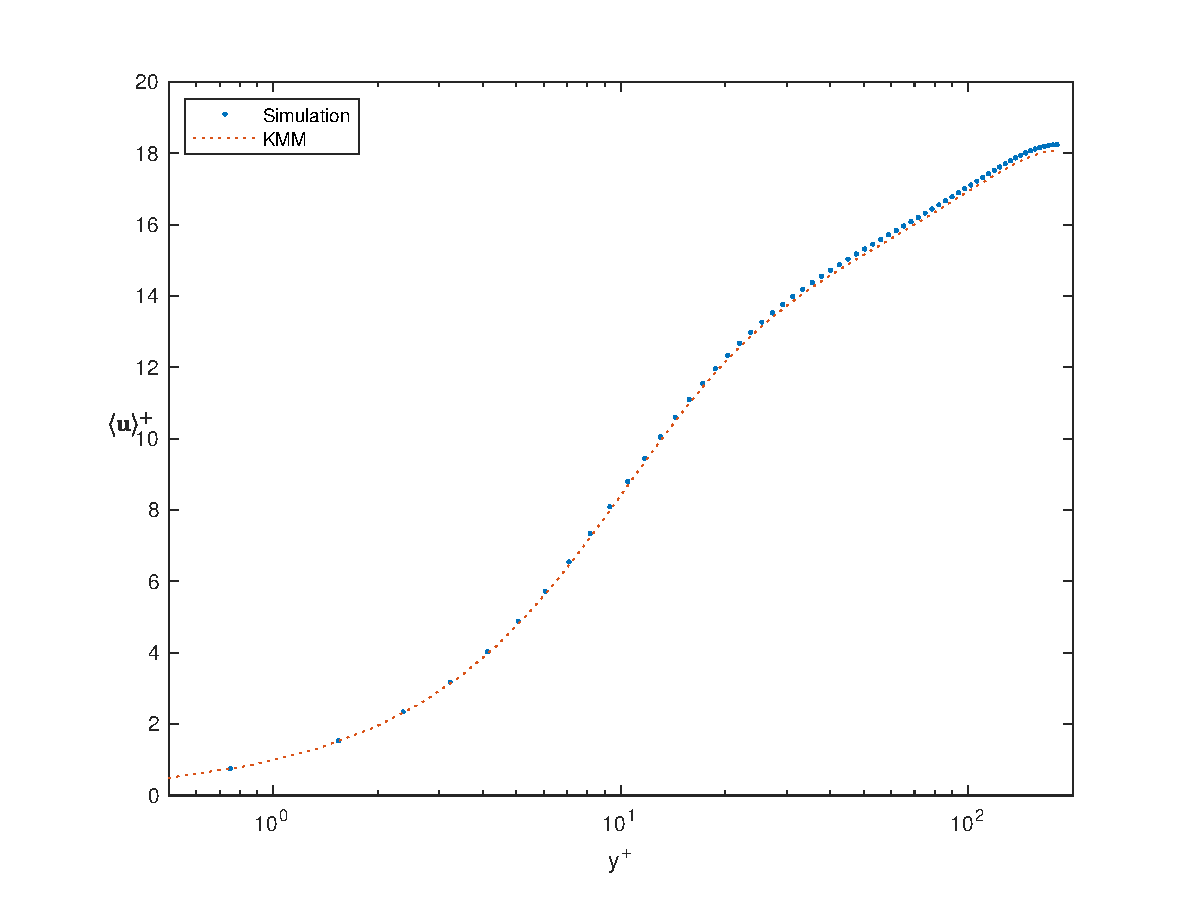
\includegraphics[scale=0.55]{grafici/loglaw_180.eps}
\caption{$\bar{u}^{+}$ in the near wall region for a $Re_{\tau}=180$ simulation}
\label{loglaw_180}
\end{center} 
\end{figure}

\begin{figure}
\begin{center}
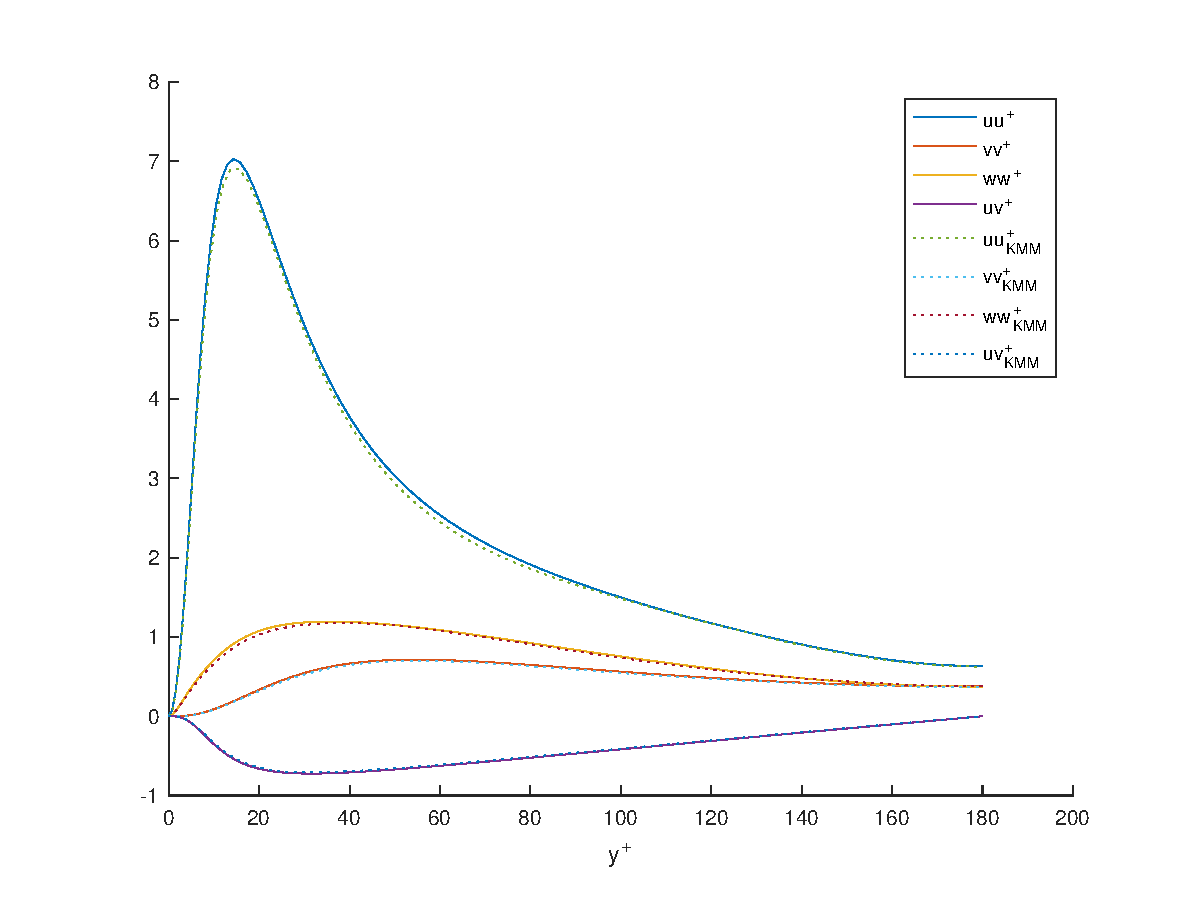
\includegraphics[scale=0.55]{grafici/budget_180.eps}
\caption{TKE budget for a $Re_{\tau}=180$ simulation}
\label{budget_180}
\end{center} 
\end{figure}


Our statistics have been registered using a simulation time of 50 non dimensional units, recording data every 0.1 steps.
In total 500 fields have been used to perform the ensemble average. \par

The data fitting is good, despite being perfect. The differences are related to the fluctuations present in the~\cite{kim_moin_moser} database, which, although well established, is far from being perfect. \\~\par

The results are in agreement with the typical curves behavior, in particular, by looking at the budget curves, we can clearly see that $\langle uu\rangle$ and $\langle ww\rangle$ increase from 0 as $y^{2}$, while $\langle uv\rangle$ and $\langle vv\rangle$ increase more slowly, as $y^{3}$ and $y^{4}$, in agreement with~\cite[284]{pope}.
All these information testify that, close to the walls, there is a \emph{two component flow}, with $v=0$ whereas $u$ and $w$ are non-zero. The resulting motion corresponds to flow in planes parallel to the wall. \\~\par

The figure~\ref{loglaw_180} report the $\bar{u}^{+}$ behavior near the wall. From 0 up to 5 $y^{+}$ units we can see the typical $\bar{u}^{+}=y^{+}$ behavior, which characterize the viscous sublayer. Once $y^{+}>30$ we see the arise of the logarithmic law of the wall, characterized by the equation

\begin{equation*}
\bar{u}^{+} = \frac{1}{\kappa} \ln y^{+} +C^{+},
\end{equation*}

where the constants $\kappa=0.41$ and $C^{+}\approx 5.2$, like smooth wall experiments, made by Von Karman, evidenced. \par
This velocity profile is typically denoted as \emph{the law of the wall}, and has been postulated by Prandtl in 1925.